\documentclass[xcolor=table,dvipsnames,table]{beamer}
\mode<presentation>
\usetheme{boxes}
\setbeamertemplate{navigation symbols}{}
% http://www.latex-community.org/forum/viewtopic.php?f=4&t=6694
\setbeamertemplate{navigation symbols}{\raisebox{5pt}{\makebox[\paperwidth]{\hfill\makebox[10pt]{\scriptsize\insertframenumber\vspace{1ex}}}}}
%\setbeamertemplate{footline}[frame number]
\setbeamertemplate{blocks}[shadow=false]
%\setbeamercolor*{block title}{fg=structure,bg=RoyalBlue!10}
\setbeamercolor*{block title example}{fg=structure,bg=RoyalBlue!10}
%\setbeamercolor*{block title example}{fg=BrickRed,bg=Goldenrod!10}
\setbeamercolor*{block title alerted}{fg=white,bg=black}
\addtobeamertemplate{block begin}{\pgfsetfillopacity{0.8}}{\pgfsetfillopacity{1}}
%\rowcolors{0}{RoyalBlue!20}{RoyalBlue!5}
\setbeamertemplate{caption}{\raggedright\insertcaption\par}

%\DeclareGraphicsRule{*}{mps}{*}{}

\usepackage{latexsym}
\usepackage{hyperref}
\usepackage{tikz}
\usetikzlibrary{calc,shapes,arrows,shadows,shapes.callouts,shapes.arrows,chains,positioning,trees}
\usepackage{solution}
\usepackage{calc}
\usepackage{pifont}
\usepackage{algorithmic}
\usepackage{pdfcomment}
\usepackage{color}

\newcommand{\cmark}{\ding{51}}
\newcommand{\xmark}{\ding{55}}

\newcommand{\highlight}[1]{{\color{blue}{#1}}}
\newcommand{\mycite}[1]{{\color{darkgray}{\footnotesize [#1]}}}

\DeclareMathOperator*{\argmin}{arg\,min}
\DeclareMathOperator*{\argmax}{arg\,max}
\DeclareMathOperator{\sign}{sign}
\DeclareMathOperator{\cnt}{Count}

\newcounter{mycallout}

\newcommand{\callouts}[3]{%
  \stepcounter{mycallout}
  \tikz[remember picture,baseline]{\node[anchor=base,inner sep=0,outer sep=0]%
    (\themycallout) {\colorbox{#1!20}{#3}};\pause\node[overlay,rectangle callout,%
    callout relative pointer={(0cm,0.5cm)},fill=#1!20] at ($(\themycallout.south)+(-0cm,-0.7cm)$){#2};}%
    }%

\raggedright

\newcount\lecturecount
\lecturecount=0
\AtBeginLecture{%
    \advance\lecturecount by 1
    \date{}
    \begin{frame}
    \begin{center}
    \titlepage
    \ifnum\lecturecount=1
    Part \the\lecturecount: \insertlecture
    \else
    Part \the\lecturecount: \insertlecture
    \fi
    \end{center}
    \end{frame}
}

\addtobeamertemplate{block begin}{\setlength\abovedisplayskip{0pt}}

%\newcommand{\example}[1]{{\color{BrickRed!50}{#1}}}
\newcommand{\maths}[1]{{\color{RoyalBlue!50}{#1}}}
\newcommand{\reference}[1]{{\color{RoyalBlue!30}\tiny [from #1]}}
\newcommand{\koehnref}{\reference{\href{http://www.statmt.org/book}{P.Koehn SMT book slides}}}


\begin{document}


\title{\color{MidnightBlue}Natural Language Processing}

\author{Anoop Sarkar \\ {\color{RoyalBlue!70}{\href{http://anoopsarkar.github.io/nlp-class}{anoopsarkar.github.io/nlp-class}}}}
\institute{\color{BrickRed}Simon Fraser University}
%\date{}
     
{
\addtocounter{framenumber}{-1}
\begin{frame}
\begin{center}
\vspace{8mm}

\includegraphics[scale=0.35]{figures/natlang-cky-logo}
\end{center}
\titlepage
\end{frame}
}



\newcommand{\tgt}{\textbf{e}}
\newcommand{\src}{\textbf{f}}
\newcommand{\aln}{\textbf{a}}

\lecture{Generative Models for Word Alignment}{}

\section{Statistical Machine Translation}
\frame{\tableofcontents[currentsection]}

\begin{frame}
\frametitle{Statistical Machine Translation}
\begin{block}{Noisy Channel Model}
\begin{eqnarray*}
\tgt^\ast & = & \arg\max_{\tgt} \underbrace{\Pr(\tgt)}_{\color{red}\textbf{Language Model}} \pause \cdot \underbrace{\Pr(\src \mid \tgt)}_{\color{blue}\textbf{Alignment Model}}
\end{eqnarray*}
\end{block}
\end{frame}

\begin{frame}
\def\blockdist{2.0}
\begin{alertblock}{Alignment Task}
\begin{tikzpicture}[node distance=2.5cm,auto,>=latex']
    \node (a) {Program};
    \path (a.140)+(-\blockdist,0) node (b) {\tgt};
    \path (a.-140)+(-\blockdist,0) node (c) {\src};
    \node (d) [right of=a] {$\Pr(\tgt \mid \src)$};
    \path[->] (b) edge (a);
    \path[->] (c) edge (a);
    \path[->] (a) edge (d);
\end{tikzpicture}
\end{alertblock}\pause
\begin{alertblock}{Training Data}
\begin{itemize}[<+->]
\item \color{blue}\textbf{Alignment Model}: learn a mapping between \src and \tgt. \\
Training data: lots of translation pairs between \src and \tgt.
\end{itemize}
\end{alertblock}
\end{frame}

\begin{frame}
\frametitle{Statistical Machine Translation}
\begin{block}{The IBM Models}
\begin{itemize}[<+->]
\item The first statistical machine translation models were developed at IBM Research (Yorktown Heights, NY) in the 1980s
\item The models were published in 1993: \\
{\small Brown et.\ al.\ The Mathematics of Statistical Machine Translation. \textit{Computational Linguistics}. 1993.} \\
{\small \url{http://aclweb.org/anthology/J/J93/J93-2003.pdf}}
\item These models are the basic SMT models, called: \\
IBM Model 1, IBM Model 2, IBM Model 3, IBM Model 4, IBM Model 5 \\
as they were called in the 1993 paper.
\item We use \tgt and \src\ in the equations in honor of their system which translated from French to English.\\
Trained on the Canadian Hansards (Parliament Proceedings)
%\item Twenty years later, they came together at a workshop called {\color{blue}\hyperlink{https://sites.google.com/site/20yearsofbitext/}{Twenty Years of Bitext}} \\
%Transcript: \url{http://cs.jhu.edu/~post/bitext/}
\end{itemize}
\end{block}
\end{frame}

\section{Generative Model of Word Alignment}
\frame{\tableofcontents[currentsection]}

\begin{frame}
\frametitle{Generative Model of Word Alignment}
\begin{block}{}
\begin{itemize}
\item English \tgt: Mary did not slap the green witch
\item ``French'' \src: Maria no daba una botefada a la bruja verde
\item Alignment \aln: $\{ 1, 3, 4, 4, 4, 5, 5, 7, 6 \}$ \\
e.g.\ $(f_8, e_{a_8})$ = $(f_8, e_7)$ = (bruja, witch)
\end{itemize}
\end{block}\pause
\begin{block}{Visualizing alignment \aln}
\begin{tikzpicture}
\begin{scope}[start chain=going right,node distance=2mm]
\def\ephr{0/{Mary},1/{did},2/{not},3/{slap},4/{the},5/{green},6/{witch}}
\foreach \i / \element in \ephr
  \node [on chain] (e\i) {\strut \element};
\end{scope}

\begin{scope}[yshift=-16mm,start chain=going right,node distance=2mm]
\def\sphr{0/{Maria},1/{no},2/{daba},3/{una},4/{botefada},5/{a},6/{la},7/{bruja},8/{verde}}
\foreach \j / \element in \sphr
  \node [on chain] (s\j) {\strut \element};
\end{scope}

\draw (e0) -- (s0);
\draw (e2) -- (s1);
\draw (e3) -- (s2);
\draw (e3) -- (s3);
\draw (e3) -- (s4);
\draw (e4) -- (s5);
\draw (e4) -- (s6);
\draw (e5) -- (s8);
\draw (e6) -- (s7);
\end{tikzpicture}

\end{block}
\end{frame}

\begin{frame}
\frametitle{Generative Model of Word Alignment}
\begin{block}{Data Set}
\begin{itemize}[<+->]
\item Data set ${\cal D}$ of $N$ sentences:
\[ {\cal D} = \{ (\src^{(1)}, \tgt^{(1)}), \ldots, (\src^{(N)}, \tgt^{(N)}) \} \]
\item French $\src$: $( f_1, f_2, \ldots, f_I )$
\item English $\tgt$: $( e_1, e_2, \ldots, e_J )$
\item Alignment $\aln$: $( a_1, a_2, \ldots, a_I )$
\item length($\src$) = length($\aln$) = $I$
\end{itemize}
\end{block}
\end{frame}

\begin{frame}
\frametitle{Generative Model of Word Alignment}
\begin{block}{Find the best alignment for each translation pair}
\[ \aln^\ast = \arg\max_{\aln} \Pr(\aln \mid \src, \tgt) \]
\end{block}\pause
\begin{block}{Alignment probability}
\begin{eqnarray*}
\Pr(\aln \mid \src, \tgt) &=& \frac{ \Pr( \src, \aln, \tgt ) }{ \Pr(\src, \tgt) }\pause\\
&=& \frac{ \Pr(\tgt) \Pr( \src, \aln \mid \tgt ) }{ \Pr(\tgt) \Pr(\src \mid \tgt) }\pause\\
&=& \frac{ \Pr( \src, \aln \mid \tgt ) }{ \Pr(\src \mid \tgt) }\pause\\
&=&\frac{ \color{red} \Pr( \src, \aln \mid \tgt ) }{ \sum_{\aln} {\color{red} \Pr(\src, \aln \mid \tgt)} }
\end{eqnarray*}
\end{block}
\end{frame}

\subsection{Word Alignments: IBM Model 3}
\frame{\tableofcontents[currentsection]}

\begin{frame}
\frametitle{Word Alignments: IBM Model 3}
\begin{block}{Generative ``story'' for $P(\src, \aln \mid \tgt)$}
\begin{tikzpicture}
\begin{scope}[start chain=going right,node distance=2mm]
\def\fphr{0/{Mary},1/{did},2/{not},3/{slap},4/{the},5/{green},6/{witch}}
\foreach \i / \element in \fphr
  \node [on chain] (k\i) {\strut \element};
\end{scope}

\begin{scope}[yshift=-16mm,start chain=going right,node distance=2mm]
\def\ephr{0/{Mary},1/{not},2/{slap},3/{slap},4/{slap},5/{the},6/{the},7/{green},8/{witch},9/{\tiny(fertility)}}
\foreach \j / \element in \ephr
  \node [on chain] (e\j) {\strut \element};
\end{scope}

\draw[->] (k0) -- (e0);
\draw[->] (k2) -- (e1);
\draw[->] (k3) -- (e2);
\draw[->] (k3) -- (e3);
\draw[->] (k3) -- (e4);
\draw[->] (k4) -- (e5);
\draw[->] (k4) -- (e6);
\draw[->] (k5) -- (e7);
\draw[->] (k6) -- (e8);

\pause 

\begin{scope}[yshift=-32mm,start chain=going right,node distance=2mm]
\def\sphr{0/{Maria},1/{no},2/{daba},3/{una},4/{botefada},5/{a},6/{la},7/{verde},8/{bruja},9/{\tiny(translate)}}
\foreach \j / \element in \sphr
  \node [on chain] (s\j) {\strut \element};
\end{scope}

\draw[->] (e0) -- (s0);
\draw[->] (e1) -- (s1);
\draw[->] (e2) -- (s2);
\draw[->] (e3) -- (s3);
\draw[->] (e4) -- (s4);
\draw[->] (e5) -- (s5);
\draw[->] (e6) -- (s6);
\draw[->] (e7) -- (s7);
\draw[->] (e8) -- (s8);

\pause

\begin{scope}[yshift=-48mm,start chain=going right,node distance=2mm]
\def\rphr{0/{Maria},1/{no},2/{daba},3/{una},4/{botefada},5/{a},6/{la},7/{bruja},8/{verde},9/{\tiny(reorder)}}
\foreach \j / \element in \rphr
  \node [on chain] (r\j) {\strut \element};
\end{scope}

\draw[->] (s0) -- (r0);
\draw[->] (s1) -- (r1);
\draw[->] (s2) -- (r2);
\draw[->] (s3) -- (r3);
\draw[->] (s4) -- (r4);
\draw[->] (s5) -- (r5);
\draw[->] (s6) -- (r6);
\draw[->] (s7) -- (r8);
\draw[->] (s8) -- (r7);

\end{tikzpicture}
\end{block}
\end{frame}

\begin{frame}
\frametitle{Word Alignments: IBM Model 3}
\begin{block}{Fertility parameter}
\[ n(\phi_j \mid e_j) : n(3 \mid \textit{slap}) ; n(0 \mid \textit{did}) \]
\end{block}\pause
\begin{block}{Translation parameter}
\[ t(f_i \mid e_{a_i}) : t(\textit{bruja} \mid \textit{witch}) \]
\end{block}\pause
\begin{block}{Distortion parameter}
\[ d(f_{\textit{pos}} = i \mid e_{\textit{pos}} = j, I, J) : d(8 \mid 7, 9, 7) \]
\end{block}
\end{frame}

\begin{frame}
\frametitle{Word Alignments: IBM Model 3}
\begin{block}{Generative model for $P(\src, \aln \mid \tgt)$}
\begin{eqnarray*}
P(\src, \aln \mid \tgt) & = & \prod_{i=1}^I n(\phi_{a_i} \mid e_{a_i})  \pause\\
& \times & t(f_i \mid e_{a_i}) \pause\\
& \times & d(i \mid a_i, I, J)
\end{eqnarray*}
\end{block}
\end{frame}

\begin{frame}
\frametitle{Word Alignments: IBM Model 3}
\begin{block}{Sentence pair with alignment $\aln = (4,3,1,2)$}
\begin{tikzpicture}

\begin{scope}[start chain=going right,node distance=2mm]
\def\ephr{1/{the},2/{house},3/{is},4/{small}}
\foreach \i / \element in \ephr
  \node [on chain] (e\i) {\strut $\stackrel{\i}{\mbox{\element}}$};
\end{scope}

\begin{scope}[yshift=-14mm,start chain=going right,node distance=2mm]
\def\dphr{1/{klein},2/{ist},3/{das},4/{Haus}}
\foreach \i / \element in \dphr
  \node [on chain] (d\i) {\strut $\stackrel{\i}{\mbox{\element}}$};
\end{scope}

\draw (e1.south) -- (d3.north);
\draw (e2.south) -- (d4.north);
\draw (e3.south) -- (d2.north);
\draw (e4.south) -- (d1.north);

\end{tikzpicture}
\end{block}\pause
If we know the parameter values we can easily compute the probability of this aligned sentence pair.
\begin{block}{$\Pr(\src, \aln \mid \tgt) = $}
\[
\begin{array}{lllll}
n(1 \mid \textrm{the}) & \times & t(\textrm{das} \mid \textrm{the}) & \times & d(3 \mid 1, 4, 4) \times \pause \\
n(1 \mid \textrm{house}) & \times & t(\textrm{Haus} \mid \textrm{house}) & \times & d(4 \mid 2, 4, 4) \times \pause \\
n(1 \mid \textrm{is}) & \times & t(\textrm{ist} \mid \textrm{is}) & \times & d(2 \mid 3, 4, 4) \times \pause \\
n(1 \mid \textrm{small}) & \times & t(\textrm{klein} \mid \textrm{small}) & \times & d(1 \mid 4, 4, 4)
\end{array}
\]
\end{block}
\end{frame}

\begin{frame}
\frametitle{Word Alignments: IBM Model 3}

\begin{columns}[t]

\begin{column}{\textwidth/2}

\begin{tikzpicture}

\begin{scope}[start chain=going right,node distance=2mm]
\def\ephr{1/{the},2/{house},3/{is},4/{small}}
\foreach \i / \element in \ephr
  \node [on chain] (e\i) {\strut $\stackrel{\i}{\mbox{\element}}$};
\end{scope}

\begin{scope}[yshift=-14mm,start chain=going right,node distance=2mm]
\def\dphr{1/{klein},2/{ist},3/{das},4/{Haus}}
\foreach \i / \element in \dphr
  \node [on chain] (d\i) {\strut $\stackrel{\i}{\mbox{\element}}$};
\end{scope}

\draw (e1.south) -- (d3.north);
\draw (e2.south) -- (d4.north);
\draw (e3.south) -- (d2.north);
\draw (e4.south) -- (d1.north);

\end{tikzpicture}

\end{column}

\begin{column}{\textwidth/2}

\begin{tikzpicture}

\begin{scope}[start chain=going right,node distance=2mm]
\def\ephr{1/{the},2/{building},3/{is},4/{small}}
\foreach \i / \element in \ephr
  \node [on chain] (e\i) {\strut $\stackrel{\i}{\mbox{\element}}$};
\end{scope}

\begin{scope}[yshift=-14mm,start chain=going right,node distance=2mm]
\def\dphr{1/{das},2/{Haus},3/{ist},4/{klein}}
\foreach \i / \element in \dphr
  \node [on chain] (d\i) {\strut $\stackrel{\i}{\mbox{\element}}$};
\end{scope}

\draw (e1.south) -- (d1.north);
\draw (e2.south) -- (d2.north);
\draw (e3.south) -- (d3.north);
\draw (e4.south) -- (d4.north);

\end{tikzpicture}

\end{column}

\end{columns}

\begin{columns}[t]

\begin{column}{\textwidth/2}

\begin{tikzpicture}

\begin{scope}[start chain=going right,node distance=2mm]
\def\ephr{1/{the},2/{home},3/{is},4/{very},5/{small}}
\foreach \i / \element in \ephr
  \node [on chain] (e\i) {\strut $\stackrel{\i}{\mbox{\element}}$};
\end{scope}

\begin{scope}[yshift=-14mm,start chain=going right,node distance=2mm]
\def\dphr{1/{das},2/{Haus},3/{ist},4/{klitzeklein}}
\foreach \i / \element in \dphr
  \node [on chain] (d\i) {\strut $\stackrel{\i}{\mbox{\element}}$};
\end{scope}

\draw (e1.south) -- (d1.north);
\draw (e2.south) -- (d2.north);
\draw (e3.south) -- (d3.north);
\draw (e5.south) -- (d4.north);

\end{tikzpicture}

\end{column}

\begin{column}{\textwidth/2}

\begin{tikzpicture}

\begin{scope}[start chain=going right,node distance=2mm]
\def\ephr{1/{the},2/{house},3/{is},4/{small}}
\foreach \i / \element in \ephr
  \node [on chain] (e\i) {\strut $\stackrel{\i}{\mbox{\element}}$};
\end{scope}

\begin{scope}[yshift=-14mm,start chain=going right,node distance=2mm]
\def\dphr{1/{das},2/{Haus},3/{ist},4/{ja},5/{klein}}
\foreach \i / \element in \dphr
  \node [on chain] (d\i) {\strut $\stackrel{\i}{\mbox{\element}}$};
\end{scope}

\draw (e1.south) -- (d1.north);
\draw (e2.south) -- (d2.north);
\draw (e3.south) -- (d3.north);
\draw (e4.south) -- (d4.north);
\draw (e4.south) -- (d5.north);

\end{tikzpicture}

\end{column}

\end{columns}\pause

\begin{block}{Parameter Estimation}
\begin{itemize}[<+->]
\item What is $n(1 \mid \textrm{very})$ = ? and $n(0 \mid \textrm{very})$ = ?
\item What is $t(\textrm{Haus} \mid \textrm{house})$ = ? and $t(\textrm{klein} \mid \textrm{small})$ = ?
\item What is $d(1 \mid 4, 4, 4)$ = ? and $d(1 \mid 1, 4, 4)$ = ?
\end{itemize}
\end{block}
\end{frame}

\begin{frame}
\frametitle{Word Alignments: IBM Model 3}

\begin{columns}[t]

\begin{column}{\textwidth/2}

\fbox{
\begin{tikzpicture}

\begin{scope}[start chain=going right,node distance=2mm]
\def\ephr{1/{the},2/{house},3/{is},4/{small}}
\foreach \i / \element in \ephr
  \node [on chain] (e\i) {\strut $\stackrel{\i}{\mbox{\element}}$};
\end{scope}

\begin{scope}[yshift=-14mm,start chain=going right,node distance=2mm]
\def\dphr{1/{klein},2/{ist},3/{das},4/{Haus}}
\foreach \i / \element in \dphr
  \node [on chain] (d\i) {\strut $\stackrel{\i}{\mbox{\element}}$};
\end{scope}

\end{tikzpicture}
}

\end{column}

\begin{column}{\textwidth/2}

\fbox{
\begin{tikzpicture}

\begin{scope}[start chain=going right,node distance=2mm]
\def\ephr{1/{the},2/{building},3/{is},4/{small}}
\foreach \i / \element in \ephr
  \node [on chain] (e\i) {\strut $\stackrel{\i}{\mbox{\element}}$};
\end{scope}

\begin{scope}[yshift=-14mm,start chain=going right,node distance=2mm]
\def\dphr{1/{das},2/{Haus},3/{ist},4/{klein}}
\foreach \i / \element in \dphr
  \node [on chain] (d\i) {\strut $\stackrel{\i}{\mbox{\element}}$};
\end{scope}

\end{tikzpicture}
}

\end{column}

\end{columns}

\begin{columns}[t]

\begin{column}{\textwidth/2}

\fbox{
\begin{tikzpicture}

\begin{scope}[start chain=going right,node distance=2mm]
\def\ephr{1/{the},2/{home},3/{is},4/{very},5/{small}}
\foreach \i / \element in \ephr
  \node [on chain] (e\i) {\strut $\stackrel{\i}{\mbox{\element}}$};
\end{scope}

\begin{scope}[yshift=-14mm,start chain=going right,node distance=2mm]
\def\dphr{1/{das},2/{Haus},3/{ist},4/{klitzeklein}}
\foreach \i / \element in \dphr
  \node [on chain] (d\i) {\strut $\stackrel{\i}{\mbox{\element}}$};
\end{scope}

\end{tikzpicture}
}

\end{column}

\begin{column}{\textwidth/2}

\fbox{
\begin{tikzpicture}

\begin{scope}[start chain=going right,node distance=2mm]
\def\ephr{1/{the},2/{house},3/{is},4/{small}}
\foreach \i / \element in \ephr
  \node [on chain] (e\i) {\strut $\stackrel{\i}{\mbox{\element}}$};
\end{scope}

\begin{scope}[yshift=-14mm,start chain=going right,node distance=2mm]
\def\dphr{1/{das},2/{Haus},3/{ist},4/{ja},5/{klein}}
\foreach \i / \element in \dphr
  \node [on chain] (d\i) {\strut $\stackrel{\i}{\mbox{\element}}$};
\end{scope}

\end{tikzpicture}
}

\end{column}

\end{columns}\pause

\begin{block}{Parameter Estimation: Sum over all alignments}
\[ \sum_{\aln} \Pr(\src, \aln \mid \tgt) = \sum_{\aln} \prod_{i=1}^I {\color{RoyalBlue} n(\phi_{a_i} \mid e_{a_i})} \times {\color{red} t(f_i \mid e_{a_i})} \times {\color{blue} d(i \mid a_i, I, J)} \]
\end{block}
\end{frame}

\begin{frame}
\frametitle{Word Alignments: IBM Model 3}
\begin{block}{Summary}
\begin{itemize}[<+->]
\item If {\color{blue} we know the parameter values} we can easily compute the probability $\Pr(\aln \mid \src, \tgt)$ given an aligned sentence pair
\item If {\color{blue} we are given a corpus of sentence pairs with alignments} we can easily learn the parameter values by using relative frequencies.
\item If we do not know the alignments then perhaps {\color{red} we can produce all possible alignments} each with a certain probability?
\end{itemize}

\end{block}\pause

\begin{block}{IBM Model 3 is too hard: Let us try learning only $t(f_i \mid e_{a_i})$}
\[ \sum_{\aln} \Pr(\src, \aln \mid \tgt) = \sum_{\aln} \prod_{i=1}^I {\color{RoyalBlue} n(\phi_{a_i} \mid e_{a_i})} \times {\color{red} t(f_i \mid e_{a_i})} \times {\color{blue} d(i \mid a_i, I, J)} \]

\end{block}


\end{frame}

\subsection{Word Alignments: IBM Model 1}
\frame{\tableofcontents[currentsection]}

\begin{frame}
\frametitle{Word Alignments: IBM Model 1}
\begin{block}{Alignment probability}
\[ \Pr(\aln \mid \src, \tgt) = \frac{ \Pr( \src, \aln \mid \tgt ) }{ \sum_{\aln} \Pr(\src, \aln \mid \tgt) } 
\]
\end{block}\pause

\begin{columns}[t]

\begin{column}{\textwidth/2}
\begin{block}{Example alignment}

\begin{tikzpicture}

\begin{scope}[start chain=going right,node distance=2mm]
\def\ephr{1/{the},2/{house},3/{is},4/{small}}
\foreach \i / \element in \ephr
  \node [on chain] (e\i) {\strut $\stackrel{\i}{\mbox{\element}}$};
\end{scope}

\begin{scope}[yshift=-14mm,start chain=going right,node distance=2mm]
\def\dphr{1/{das},2/{Haus},3/{ist},4/{klein}}
\foreach \i / \element in \dphr
  \node [on chain] (d\i) {\strut $\stackrel{\i}{\mbox{\element}}$};
\end{scope}

\draw (e1.south) -- (d1.north);
\draw (e2.south) -- (d2.north);
\draw (e3.south) -- (d3.north);
\draw (e4.south) -- (d4.north);

\end{tikzpicture}

\end{block}
\end{column}\pause

\begin{column}{\textwidth/2}
\begin{block}{$\Pr(\src, \aln \mid \tgt) = \prod_{i=1}^I t(f_i \mid e_{a_i})$}
\begin{eqnarray*}
\lefteqn{\Pr( \src, \aln \mid \tgt ) =}\\
&& t(\textrm{das} \mid \textrm{the}) \times \\
&& t(\textrm{Haus} \mid \textrm{house}) \times \\
&& t(\textrm{ist} \mid \textrm{is}) \times \\
&& t(\textrm{klein} \mid \textrm{small})
\end{eqnarray*}
\end{block}
\end{column}

\end{columns}
\end{frame}

\begin{frame}
\frametitle{Word Alignments: IBM Model 1}
\begin{block}{Generative ``story'' for Model 1}

\begin{tikzpicture}

\begin{scope}[start chain=going right,node distance=2mm]
\def\ephr{1/{the},2/{house},3/{is},4/{small}}
\foreach \i / \element in \ephr
  \node [on chain] (e\i) {\strut \element};
\end{scope}

\begin{scope}[yshift=-14mm,start chain=going right,node distance=2mm]
\def\dphr{1/{das},2/{Haus},3/{ist},4/{klein},5/{\tiny(translate)}}
\foreach \i / \element in \dphr
  \node [on chain] (d\i) {\strut \element};
\end{scope}

\draw[->] (e1.south) -- (d1.north);
\draw[->] (e2.south) -- (d2.north);
\draw[->] (e3.south) -- (d3.north);
\draw[->] (e4.south) -- (d4.north);

\end{tikzpicture}

\[ \Pr(\src, \aln \mid \tgt) = \prod_{i=1}^I t(f_i \mid e_{a_i}) \]

\end{block}
\end{frame}

\subsection{Finding the best alignment: IBM Model 1}
\frame{\tableofcontents[currentsection]}

\begin{frame}
\frametitle{Finding the best word alignment: IBM Model 1}

\begin{block}{Compute the $\arg\max$ word alignment}
\[ \hat{\textbf{a}} = \arg\max_{\textbf{a}} \Pr(\textbf{a} \mid \textbf{e}, \textbf{f}) \]

\begin{itemize}[<+->]
\item For each $f_i$ in $(f_1, \ldots, f_I)$ build $\aln = (\hat{a_1}, \ldots, \hat{a_I})$

\[ \hat{a_i} = \arg\max_{a_i} t(f_i \mid e_{a_i}) \]
\end{itemize}
\end{block}\pause

\begin{columns}[t]

\begin{column}{\textwidth/2}
\begin{block}{Many to one alignment \cmark}

\begin{tikzpicture}

\begin{scope}[start chain=going right,node distance=2mm]
\def\ephr{1/{the},2/{house},3/{is},4/{small}}
\foreach \i / \element in \ephr
  \node [on chain] (e\i) {\strut $\stackrel{\i}{\mbox{\element}}$};
\end{scope}

\begin{scope}[yshift=-14mm,start chain=going right,node distance=2mm]
\def\dphr{1/{das},2/{Haus},3/{ist},4/{klein}}
\foreach \i / \element in \dphr
  \node [on chain] (d\i) {\strut $\stackrel{\i}{\mbox{\element}}$};
\end{scope}

\draw (e2.south) -- (d1.north);
\draw (e2.south) -- (d2.north);
\draw (e2.south) -- (d3.north);
\draw (e2.south) -- (d4.north);

\end{tikzpicture}

\end{block}
\end{column}\pause

\begin{column}{\textwidth/2}

\begin{block}{One to many alignment \xmark}

\begin{tikzpicture}

\begin{scope}[start chain=going right,node distance=2mm]
\def\ephr{1/{the},2/{house},3/{is},4/{small}}
\foreach \i / \element in \ephr
  \node [on chain] (e\i) {\strut $\stackrel{\i}{\mbox{\element}}$};
\end{scope}

\begin{scope}[yshift=-14mm,start chain=going right,node distance=2mm]
\def\dphr{1/{das},2/{Haus},3/{ist},4/{klein}}
\foreach \i / \element in \dphr
  \node [on chain] (d\i) {\strut $\stackrel{\i}{\mbox{\element}}$};
\end{scope}

\draw (e1.south) -- (d2.north);
\draw (e2.south) -- (d2.north);
\draw (e3.south) -- (d2.north);
\draw (e4.south) -- (d2.north);

\end{tikzpicture}

\end{block}

\end{column}

\end{columns}

\end{frame}

\subsection{Learning Parameters: IBM Model 1}
\frame{\tableofcontents[currentsection]}

\begin{frame}
\frametitle{Learning parameters\koehnref}
\begin{itemize}[<+->]
\item We would like to estimate the lexical translation probabilities \maths{$t(e|f)$} from a parallel corpus
\item ... but we do not have the alignments
\item Chicken and egg problem
\begin{itemize}
\item if we had the {\em alignments},\\ $\rightarrow$ we could estimate the {\em parameters} of our generative model\\[-3mm]
\item if we had the {\em parameters},\\ $\rightarrow$ we could estimate the {\em alignments}
\end{itemize}
\end{itemize}

\end{frame}

\begin{frame}
\frametitle{EM Algorithm\koehnref}
\begin{block}{}
\begin{itemize}[<+->]
\item Incomplete data
\begin{itemize}
\item if we had {\em complete data}, we could estimate {\em model}
\item if we had {\em model}, we could fill in the {\em gaps in the data}
\end{itemize}
\item Expectation Maximization (EM) in a nutshell
\begin{enumerate}
\item initialize model parameters (e.g. uniform)
\item assign probabilities to the missing data
\item estimate model parameters from completed data
\item iterate steps 2--3 until convergence 
\end{enumerate}
\end{itemize}
\end{block}

\end{frame}

\begin{frame}
\frametitle{EM Algorithm\koehnref}
\begin{center}
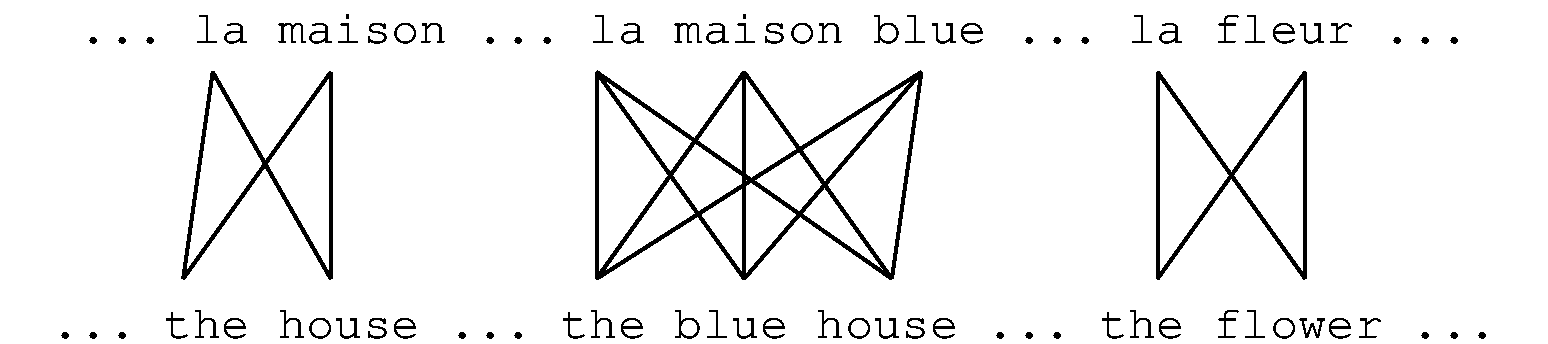
\includegraphics[scale=0.4]{figures/em1.pdf}
\end{center}
\begin{itemize}
\item Initial step: all alignments equally likely
\item Model learns that, e.g., \textit{la} is often aligned with \textit{the}
\end{itemize}

\end{frame}

\begin{frame}
\frametitle{EM Algorithm\koehnref}
\begin{center}
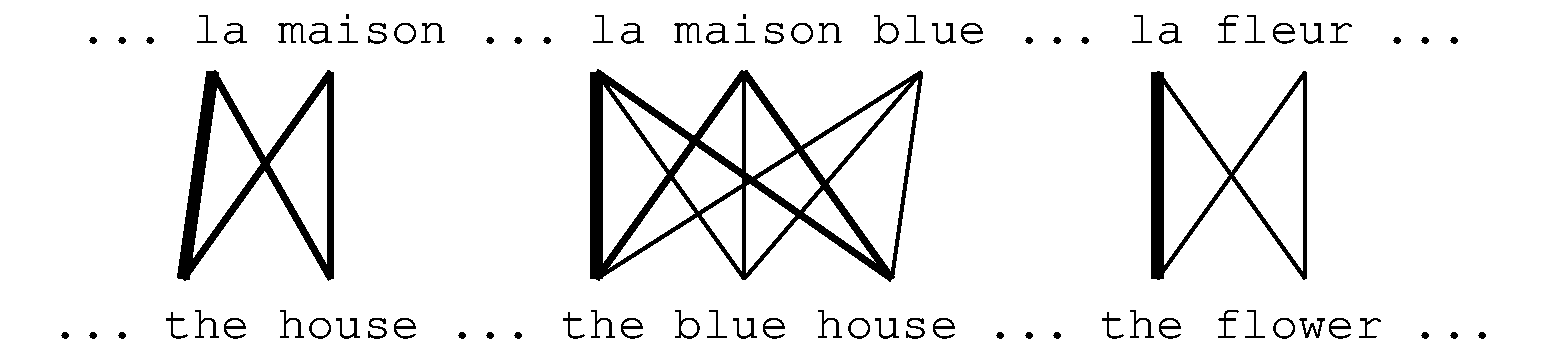
\includegraphics[scale=0.4]{figures/em2.pdf}
\end{center}
\begin{itemize}
\item After one iteration
\item Alignments, e.g., between \textit{la} and \textit{the} are more likely
\end{itemize}

\end{frame}

\begin{frame}
\frametitle{EM Algorithm\koehnref}
\begin{center}
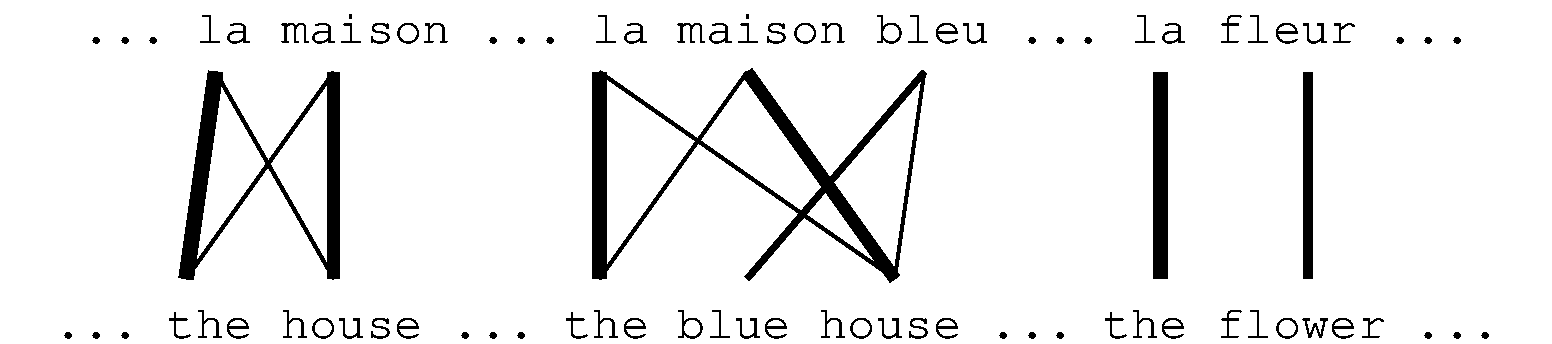
\includegraphics[scale=0.4]{figures/em3.pdf}
\end{center}
\begin{itemize}
\item After another iteration
\item It becomes apparent that alignments, e.g., between \textit{fleur}
  and \textit{flower} are more likely (pigeon hole principle)
\end{itemize}

\end{frame}

\begin{frame}
\frametitle{EM Algorithm\koehnref}

\begin{center}
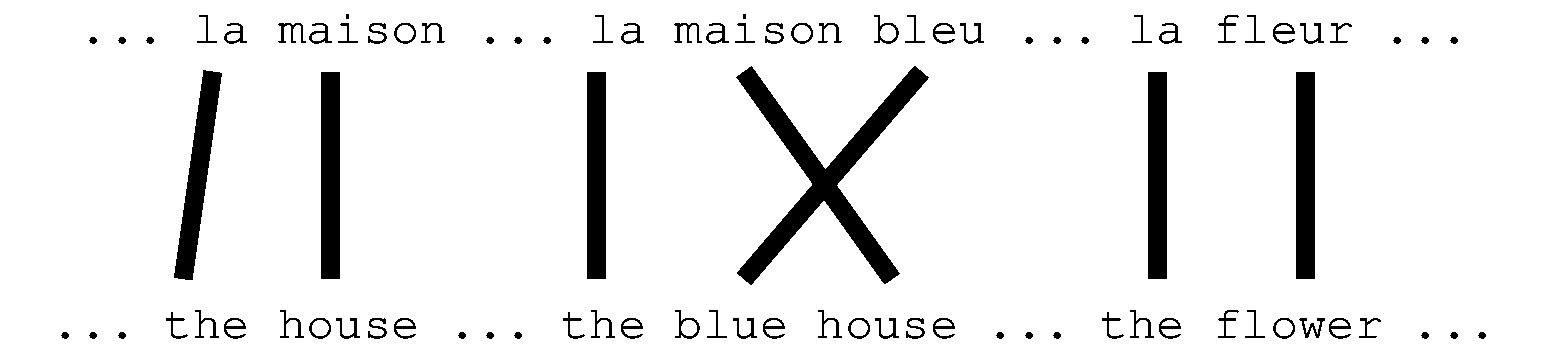
\includegraphics[scale=0.4]{figures/em4.pdf}
\end{center}
\begin{itemize}
\item Convergence
\item Inherent hidden structure revealed by EM
\end{itemize}

\end{frame}

\begin{frame}
\frametitle{EM Algorithm\koehnref}

\begin{center}
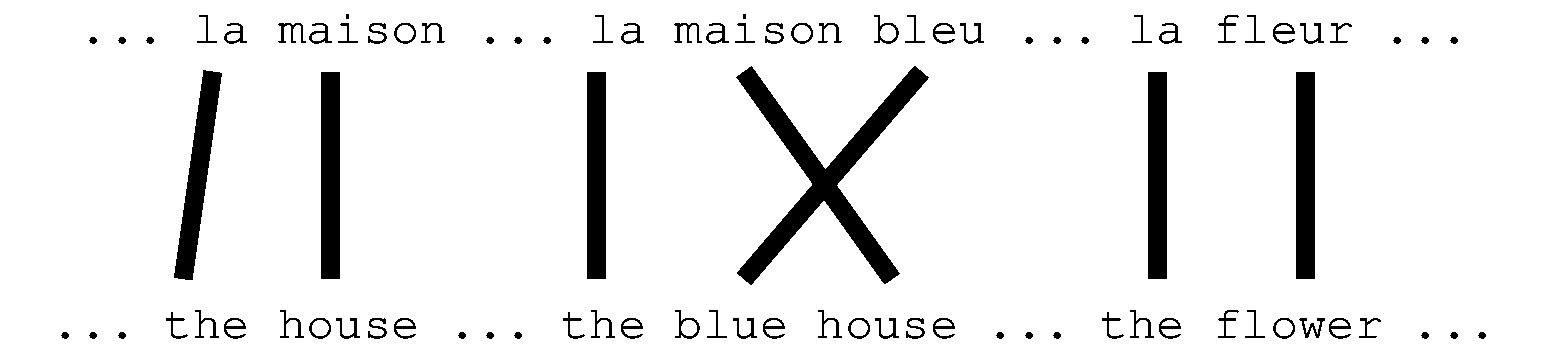
\includegraphics[scale=0.4]{figures/em4.pdf} \\
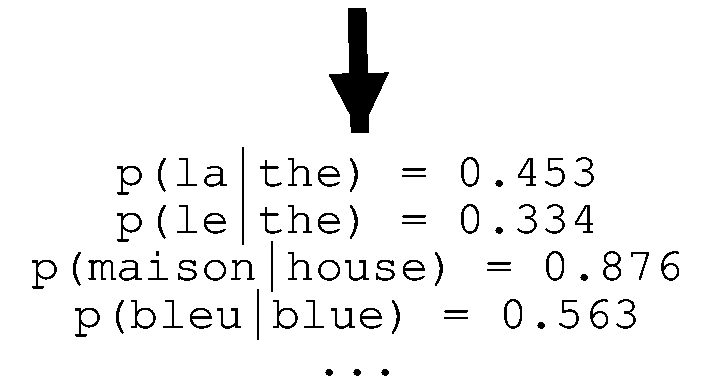
\includegraphics[scale=0.4]{figures/em-result.pdf}
\end{center}
\begin{itemize}
\item Parameter estimation from the aligned corpus
\end{itemize}

\end{frame}

\begin{frame}
\frametitle{IBM Model 1 and the EM Algorithm\koehnref}

\begin{itemize}[<+->]
\item EM Algorithm consists of two steps
\item Expectation-Step: Apply model to the data
\begin{itemize}
\item parts of the model are hidden (here: alignments)
\item using the model, assign probabilities to possible values
\end{itemize}
\item Maximization-Step: Estimate model from data
\begin{itemize}
\item take assign values as fact
\item collect counts (weighted by probabilities)
\item estimate model from counts
\end{itemize}
\item Iterate these steps until convergence
\end{itemize}

\end{frame}


\begin{frame}
\frametitle{IBM Model 1 and the EM Algorithm\koehnref}

\begin{itemize}[<+->]
\item We need to be able to compute:
\begin{itemize}
\item Expectation-Step: probability of alignments
\item Maximization-Step: count collection
\end{itemize}
\end{itemize}

\end{frame}


\begin{frame}
\frametitle{Word Alignments: IBM Model 1}
\begin{block}{Alignment probability}
\begin{eqnarray*}
\Pr(\aln \mid \src, \tgt) & = & \frac{ \Pr( \src, \aln \mid \tgt ) }{ \Pr(\src \mid \tgt) } \pause\\
& = & \frac{ \Pr( \src, \aln \mid \tgt ) }{ \sum_{\aln} \Pr(\src, \aln \mid \tgt) } \pause\\
& = & \frac{ \prod_{i=1}^I t(f_i \mid e_{a_i}) }{ \sum_{\aln} \prod_{i=1}^I t(f_i \mid e_{a_i}) }
\end{eqnarray*}
\end{block}\pause 

\begin{block}{Computing the denominator}
\begin{itemize}
\item The denominator above is summing over $J^I$ alignments
\item An interlude on how compute the denominator faster ...
\end{itemize}

\end{block}

\end{frame}

%\begin{frame}
%\frametitle{Parameter Estimation: IBM Model 1}
%\begin{block}{}
%
%\[
%t_k(f_i \mid e_j) = \sum_{s=1}^N \sum_{(f_i, e_j) \in (\textbf{f}^{(s)}, \textbf{e}^{(s)})} \frac{ \textrm{count}(f_i, e_j, \textbf{f}^{(s)}, \textbf{e}^{(s)}) }{ \textrm{count}(e_j, \textbf{f}^{(s)}, \textbf{e}^{(s)}) }
%\]
%
%\[
%\begin{eqnarray*}
%\textrm{count}(f_i, e_j, \textbf{f}, \textbf{e}) & = & \frac{ t_{k-1}(f_i \mid e_j) }{ \Pr(\textbf{f} \mid \textbf{e}, t_{k-1}) } \\
%& = & \frac{ t_{k-1}(f_i \mid e_j) }{ \sum_{a_i=1}^J t_{k-1}(f_i \mid e_{a_i}) } \\
%\textrm{count}(e_j, \textbf{f}, \textbf{e}) & = & \sum_{i=1}^I \textrm{count}(f_i, e_j, \textbf{f}, \textbf{e})
%\end{eqnarray*}
%\]
%
%\end{block}
%\end{frame}


\begin{frame}
\frametitle{Word Alignments: IBM Model 1}
\begin{block}{Sum over all alignments}
\begin{eqnarray*}
\sum_{\aln} \Pr(\src, \aln \mid \tgt) & = & 
\sum_{a_1 = 1}^J \sum_{a_2 = 1}^J \ldots \sum_{a_I = 1}^J \prod_{i=1}^I t(f_i \mid e_{a_i}) 
\end{eqnarray*}
\end{block}\pause
\begin{block}{Assume $(f_1, f_2, f_3)$ and $(e_1, e_2)$}
\[ \sum_{a_1=1}^2 \sum_{a_2=1}^2 \sum_{a_3=1}^2 t(f_1 \mid e_{a_1}) \times t(f_2 \mid e_{a_2}) \times t(f_3 \mid e_{a_3}) \]
\end{block}
\end{frame}

\begin{frame}
\frametitle{Word Alignments: IBM Model 1}
\begin{block}{Assume $(f_1, f_2, f_3)$ and $(e_1, e_2)$: $I=3$ and $J=2$}
\[ \sum_{a_1=1}^2 \sum_{a_2=1}^2 \sum_{a_3=1}^2 t(f_1 \mid e_{a_1}) \times t(f_2 \mid e_{a_2}) \times t(f_3 \mid e_{a_3}) \]
\end{block}
\begin{block}{$J^I = 2^3$ terms to be added:}
\[ 
\begin{array}{cccccc}
\color{red} t(f_1 \mid e_1) & \times & \color{red} t(f_2 \mid e_1) & \times & \color{red} t(f_3 \mid e_1) & + \\
\color{red} t(f_1 \mid e_1) & \times & \color{red} t(f_2 \mid e_1) & \times & \color{red} t(f_3 \mid e_2) & + \\
\color{blue} t(f_1 \mid e_1) & \times & \color{blue} t(f_2 \mid e_2) & \times & \color{blue} t(f_3 \mid e_1) & + \\
\color{blue} t(f_1 \mid e_1) & \times & \color{blue} t(f_2 \mid e_2) & \times & \color{blue} t(f_3 \mid e_2) & + \\
\color{red} t(f_1 \mid e_2) & \times & \color{red} t(f_2 \mid e_1) & \times & \color{red} t(f_3 \mid e_1) & + \\
\color{red} t(f_1 \mid e_2) & \times & \color{red} t(f_2 \mid e_1) & \times & \color{red} t(f_3 \mid e_2) & + \\
\color{blue} t(f_1 \mid e_2) & \times & \color{blue} t(f_2 \mid e_2) & \times & \color{blue} t(f_3 \mid e_1) & + \\
\color{blue} t(f_1 \mid e_2) & \times & \color{blue} t(f_2 \mid e_2) & \times & \color{blue} t(f_3 \mid e_2) & \\
\end{array}
\]
\end{block}
\end{frame}

\begin{frame}
\frametitle{Word Alignments: IBM Model 1}
\begin{block}{Factor the terms:}
\[ 
\begin{array}{cccc}
( t(f_1 \mid e_1) \times t(f_2 \mid e_1) ) & \times & ( t(f_3 \mid e_1) + t(f_3 \mid e_2) ) & + \\
( t(f_1 \mid e_1) \times t(f_2 \mid e_2) ) & \times & ( t(f_3 \mid e_1) + t(f_3 \mid e_2) ) & + \\
( t(f_1 \mid e_2) \times t(f_2 \mid e_1) ) & \times & ( t(f_3 \mid e_1) + t(f_3 \mid e_2) ) & + \\
( t(f_1 \mid e_2) \times t(f_2 \mid e_2) ) & \times & ( t(f_3 \mid e_1) + t(f_3 \mid e_2) ) & 
\end{array}
\]
\pause
\[ \left( t(f_3 \mid e_1) + t(f_3 \mid e_2) \right) \left(
\begin{array}{cccc}
 t(f_1 \mid e_1) & \times & t(f_2 \mid e_1)  & + \\
 t(f_1 \mid e_1) & \times & t(f_2 \mid e_2)  & + \\
 t(f_1 \mid e_2) & \times & t(f_2 \mid e_1)  & + \\
 t(f_1 \mid e_2) & \times & t(f_2 \mid e_2)  & 
\end{array}
\right) \]
\pause
\[ {\color{RoyalBlue} \left( t(f_3 \mid e_1) + t(f_3 \mid e_2) \right) } \left(
\begin{array}{cccc}
 \color{red} t(f_1 \mid e_1) & \times & \color{blue} ( t(f_2 \mid e_1) + t(f_2 \mid e_2) ) & + \\
 \color{red} t(f_1 \mid e_2) & \times & \color{blue} ( t(f_2 \mid e_1) + t(f_2 \mid e_2) ) &
\end{array}
\right) \]
\end{block}
\end{frame}

\begin{frame}
\frametitle{Word Alignments: IBM Model 1}
\begin{block}{Assume $(f_1, f_2, f_3)$ and $(e_1, e_2)$: $I=3$ and $J=2$}
\[ \prod_{i=1}^3 \sum_{a_i=1}^2 t(f_i \mid e_{a_i}) \]
\end{block}
\begin{block}{$I \times J = 2 \times 3$ terms to be added:}
\[ 
\begin{array}{cccc}
\color{red} ( t(f_1 \mid e_1) & + & \color{red} t(f_1 \mid e_2) ) & \times \\
\color{blue} ( t(f_2 \mid e_1) & + & \color{blue} t(f_2 \mid e_2) ) & \times \\
\color{RoyalBlue} ( t(f_3 \mid e_1) & + & \color{RoyalBlue} t(f_3 \mid e_2) ) & 
\end{array}
\]
\end{block}

\end{frame}

\begin{frame}
\frametitle{Word Alignments: IBM Model 1}
\begin{block}{Alignment probability}
\begin{eqnarray*}
\Pr(\aln \mid \src, \tgt) & = & \frac{ \Pr( \src, \aln \mid \tgt ) }{ \Pr(\src \mid \tgt) } \\
& = & \frac{ \prod_{i=1}^I t(f_i \mid e_{a_i}) }{ \sum_{\aln} \prod_{i=1}^I t(f_i \mid e_{a_i}) } \pause\\
& = & \frac{ \prod_{i=1}^I t(f_i \mid e_{a_i}) }{ \prod_{i=1}^I \sum_{j=1}^J t(f_i \mid e_j) }
\end{eqnarray*}
\end{block}

\end{frame}

\begin{frame}
\frametitle{Learning Parameters: IBM Model 1}

\begin{columns}[t]

\begin{column}{\textwidth/3}

\begin{tikzpicture}

\begin{scope}[start chain=going right,node distance=2mm]
\def\ephr{1/{the},2/{house}}
\foreach \i / \element in \ephr
  \node [on chain] (e\i) {\strut $\stackrel{\i}{\mbox{\element}}$};
\end{scope}

\begin{scope}[yshift=-14mm,start chain=going right,node distance=2mm]
\def\dphr{1/{das},2/{Haus}}
\foreach \i / \element in \dphr
  \node [on chain] (d\i) {\strut $\stackrel{\i}{\mbox{\element}}$};
\end{scope}

\draw (e1.south) -- (d1.north);
\draw (e2.south) -- (d2.north);

\end{tikzpicture}

\end{column}

\begin{column}{\textwidth/3}

\begin{tikzpicture}

\begin{scope}[start chain=going right,node distance=2mm]
\def\ephr{1/{the},2/{book}}
\foreach \i / \element in \ephr
  \node [on chain] (e\i) {\strut $\stackrel{\i}{\mbox{\element}}$};
\end{scope}

\begin{scope}[yshift=-14mm,start chain=going right,node distance=2mm]
\def\dphr{1/{das},2/{Buch}}
\foreach \i / \element in \dphr
  \node [on chain] (d\i) {\strut $\stackrel{\i}{\mbox{\element}}$};
\end{scope}

\draw (e1.south) -- (d1.north);
\draw (e2.south) -- (d2.north);

\end{tikzpicture}

\end{column}

\begin{column}{\textwidth/3}

\begin{tikzpicture}

\begin{scope}[start chain=going right,node distance=2mm]
\def\ephr{1/{a},2/{book}}
\foreach \i / \element in \ephr
  \node [on chain] (e\i) {\strut $\stackrel{\i}{\mbox{\element}}$};
\end{scope}

\begin{scope}[yshift=-14mm,start chain=going right,node distance=2mm]
\def\dphr{1/{ein},2/{Buch}}
\foreach \i / \element in \dphr
  \node [on chain] (d\i) {\strut $\stackrel{\i}{\mbox{\element}}$};
\end{scope}

\draw (e1.south) -- (d1.north);
\draw (e2.south) -- (d2.north);

\end{tikzpicture}

\end{column}

\end{columns}\pause

\begin{block}{Learning parameters $t(f|e)$ when alignments are known}
\[ 
 \begin{array}{cc}
 t(das \mid the) = \frac{c(das, the)}{\sum_f c(f, the)} & t(house \mid Haus) = \frac{c(Haus, house)}{\sum_f c(f, house)} \\
 t(ein \mid a) = \frac{c(ein, a)}{\sum_f c(f, a)} & t(Buch \mid book) = \frac{c(Buch, book)}{\sum_f c(f, book)}
 \end{array}
\]
\[ t(f | e) = \sum_{s=1}^N \sum_{f \rightarrow e \in \src^{(s)}, \tgt^{(s)}} \frac{ c(f, e) }{ \sum_f c(f, e) } \]
\end{block}

\end{frame}

\begin{frame}
\frametitle{Learning Parameters: IBM Model 1}

\begin{columns}[t]

\begin{column}{\textwidth/3}

\begin{tikzpicture}

\begin{scope}[start chain=going right,node distance=2mm]
\def\ephr{1/{the},2/{house}}
\foreach \i / \element in \ephr
  \node [on chain] (e\i) {\strut $\stackrel{\i}{\mbox{\element}}$};
\end{scope}

\begin{scope}[yshift=-14mm,start chain=going right,node distance=2mm]
\def\dphr{1/{das},2/{Haus}}
\foreach \i / \element in \dphr
  \node [on chain] (d\i) {\strut $\stackrel{\i}{\mbox{\element}}$};
\end{scope}

\draw[dashed] (e1.south) -- (d1.north);
\draw[dashed] (e1.south) -- (d2.north);
\draw[dashed] (e2.south) -- (d1.north);
\draw[dashed] (e2.south) -- (d2.north);

\end{tikzpicture}

\end{column}

\begin{column}{\textwidth/3}

\begin{tikzpicture}

\begin{scope}[start chain=going right,node distance=2mm]
\def\ephr{1/{the},2/{book}}
\foreach \i / \element in \ephr
  \node [on chain] (e\i) {\strut $\stackrel{\i}{\mbox{\element}}$};
\end{scope}

\begin{scope}[yshift=-14mm,start chain=going right,node distance=2mm]
\def\dphr{1/{das},2/{Buch}}
\foreach \i / \element in \dphr
  \node [on chain] (d\i) {\strut $\stackrel{\i}{\mbox{\element}}$};
\end{scope}

\draw[dashed] (e1.south) -- (d1.north);
\draw[dashed] (e1.south) -- (d2.north);
\draw[dashed] (e2.south) -- (d1.north);
\draw[dashed] (e2.south) -- (d2.north);

\end{tikzpicture}

\end{column}

\begin{column}{\textwidth/3}

\begin{tikzpicture}

\begin{scope}[start chain=going right,node distance=2mm]
\def\ephr{1/{a},2/{book}}
\foreach \i / \element in \ephr
  \node [on chain] (e\i) {\strut $\stackrel{\i}{\mbox{\element}}$};
\end{scope}

\begin{scope}[yshift=-14mm,start chain=going right,node distance=2mm]
\def\dphr{1/{ein},2/{Buch}}
\foreach \i / \element in \dphr
  \node [on chain] (d\i) {\strut $\stackrel{\i}{\mbox{\element}}$};
\end{scope}

\draw[dashed] (e1.south) -- (d1.north);
\draw[dashed] (e1.south) -- (d2.north);
\draw[dashed] (e2.south) -- (d1.north);
\draw[dashed] (e2.south) -- (d2.north);

\end{tikzpicture}

\end{column}

\end{columns}\pause

\begin{block}{Learning parameters $t(f|e)$ when alignments are {\em unknown}}

\begin{columns}[t]

\begin{column}{\textwidth/4}

\begin{tikzpicture}

\begin{scope}[start chain=going right,node distance=2mm]
\def\ephr{1/{the},2/{house}}
\foreach \i / \element in \ephr
  \node [on chain] (e\i) {\strut $\stackrel{\i}{\mbox{\element}}$};
\end{scope}

\begin{scope}[yshift=-14mm,start chain=going right,node distance=2mm]
\def\dphr{1/{das},2/{Haus}}
\foreach \i / \element in \dphr
  \node [on chain] (d\i) {\strut $\stackrel{\i}{\mbox{\element}}$};
\end{scope}

\draw (d1.north) -- (e1.south);
\draw (d2.north) -- (e1.south);

\end{tikzpicture}

\end{column}

\begin{column}{\textwidth/4}

\begin{tikzpicture}

\begin{scope}[start chain=going right,node distance=2mm]
\def\ephr{1/{the},2/{house}}
\foreach \i / \element in \ephr
  \node [on chain] (e\i) {\strut $\stackrel{\i}{\mbox{\element}}$};
\end{scope}

\begin{scope}[yshift=-14mm,start chain=going right,node distance=2mm]
\def\dphr{1/{das},2/{Haus}}
\foreach \i / \element in \dphr
  \node [on chain] (d\i) {\strut $\stackrel{\i}{\mbox{\element}}$};
\end{scope}

\draw (d1.north) -- (e1.south);
\draw (d2.north) -- (e2.south);

\end{tikzpicture}

\end{column}

\begin{column}{\textwidth/4}

\begin{tikzpicture}

\begin{scope}[start chain=going right,node distance=2mm]
\def\ephr{1/{the},2/{house}}
\foreach \i / \element in \ephr
  \node [on chain] (e\i) {\strut $\stackrel{\i}{\mbox{\element}}$};
\end{scope}

\begin{scope}[yshift=-14mm,start chain=going right,node distance=2mm]
\def\dphr{1/{das},2/{Haus}}
\foreach \i / \element in \dphr
  \node [on chain] (d\i) {\strut $\stackrel{\i}{\mbox{\element}}$};
\end{scope}

\draw (d1.north) -- (e2.south);
\draw (d2.north) -- (e1.south);

\end{tikzpicture}

\end{column}

\begin{column}{\textwidth/4}

\begin{tikzpicture}

\begin{scope}[start chain=going right,node distance=2mm]
\def\ephr{1/{the},2/{house}}
\foreach \i / \element in \ephr
  \node [on chain] (e\i) {\strut $\stackrel{\i}{\mbox{\element}}$};
\end{scope}

\begin{scope}[yshift=-14mm,start chain=going right,node distance=2mm]
\def\dphr{1/{das},2/{Haus}}
\foreach \i / \element in \dphr
  \node [on chain] (d\i) {\strut $\stackrel{\i}{\mbox{\element}}$};
\end{scope}

\draw (d1.north) -- (e2.south);
\draw (d2.north) -- (e2.south);

\end{tikzpicture}

\end{column}

\end{columns}

Also list alignments for \textit{(the book, das Buch)} and \textit{(a book, ein Buch)}

\end{block}

\end{frame}

\begin{frame}
\frametitle{Learning Parameters: IBM Model 1}

\begin{block}{Initialize $t^0(f|e)$}
\begin{columns}

\begin{column}{\textwidth/2}
\[
\begin{array}{ccc}
t(Haus \mid the) & = & 0.25 \\
t(das \mid the) & = & 0.5 \\
t(Buch \mid the) & = & 0.25 
\end{array}
\]

\end{column}

\begin{column}{\textwidth/2}
\[
\begin{array}{ccc}
t(das \mid house) & = & 0.5 \\
t(Haus \mid house) & = & 0.5 \\
t(Buch \mid house) & = & 0.0 
 \end{array}
\]

\end{column}

\end{columns}

\end{block}\pause

\begin{block}{Compute posterior for each alignment}

\begin{columns}[t]

\begin{column}{\textwidth/4}

\begin{tikzpicture}

\begin{scope}[start chain=going right,node distance=2mm]
\def\ephr{1/{the},2/{house}}
\foreach \i / \element in \ephr
  \node [on chain] (e\i) {\strut $\stackrel{\i}{\mbox{\element}}$};
\end{scope}

\begin{scope}[yshift=-14mm,start chain=going right,node distance=2mm]
\def\dphr{1/{das},2/{Haus}}
\foreach \i / \element in \dphr
  \node [on chain] (d\i) {\strut $\stackrel{\i}{\mbox{\element}}$};
\end{scope}

\draw (d1.north) -- (e1.south);
\draw (d2.north) -- (e1.south);

\end{tikzpicture}

\end{column}

\begin{column}{\textwidth/4}

\begin{tikzpicture}

\begin{scope}[start chain=going right,node distance=2mm]
\def\ephr{1/{the},2/{house}}
\foreach \i / \element in \ephr
  \node [on chain] (e\i) {\strut $\stackrel{\i}{\mbox{\element}}$};
\end{scope}

\begin{scope}[yshift=-14mm,start chain=going right,node distance=2mm]
\def\dphr{1/{das},2/{Haus}}
\foreach \i / \element in \dphr
  \node [on chain] (d\i) {\strut $\stackrel{\i}{\mbox{\element}}$};
\end{scope}

\draw (d1.north) -- (e1.south);
\draw (d2.north) -- (e2.south);

\end{tikzpicture}

\end{column}

\begin{column}{\textwidth/4}

\begin{tikzpicture}

\begin{scope}[start chain=going right,node distance=2mm]
\def\ephr{1/{the},2/{house}}
\foreach \i / \element in \ephr
  \node [on chain] (e\i) {\strut $\stackrel{\i}{\mbox{\element}}$};
\end{scope}

\begin{scope}[yshift=-14mm,start chain=going right,node distance=2mm]
\def\dphr{1/{das},2/{Haus}}
\foreach \i / \element in \dphr
  \node [on chain] (d\i) {\strut $\stackrel{\i}{\mbox{\element}}$};
\end{scope}

\draw (d1.north) -- (e2.south);
\draw (d2.north) -- (e1.south);

\end{tikzpicture}

\end{column}

\begin{column}{\textwidth/4}

\begin{tikzpicture}

\begin{scope}[start chain=going right,node distance=2mm]
\def\ephr{1/{the},2/{house}}
\foreach \i / \element in \ephr
  \node [on chain] (e\i) {\strut $\stackrel{\i}{\mbox{\element}}$};
\end{scope}

\begin{scope}[yshift=-14mm,start chain=going right,node distance=2mm]
\def\dphr{1/{das},2/{Haus}}
\foreach \i / \element in \dphr
  \node [on chain] (d\i) {\strut $\stackrel{\i}{\mbox{\element}}$};
\end{scope}

\draw (d1.north) -- (e2.south);
\draw (d2.north) -- (e2.south);

\end{tikzpicture}

\end{column}

\end{columns}

\[
\Pr(\aln \mid \src, \tgt) 
= \frac{ \Pr( \src, \aln \mid \tgt ) }{ \Pr(\src \mid \tgt) } 
= \frac{ \prod_{i=1}^I t(f_i \mid e_{a_i}) }{ \prod_{i=1}^I \sum_{j=1}^J t(f_i \mid e_j) }
\]

\end{block}

\end{frame}

\begin{frame}
\frametitle{Learning Parameters: IBM Model 1}

\begin{block}{Initialize $t^0(f|e)$}
\begin{columns}

\begin{column}{\textwidth/2}
\[
\begin{array}{ccc}
t(Haus \mid the) & = & 0.25 \\
t(das \mid the) & = & 0.5 \\
t(Buch \mid the) & = & 0.25 
\end{array}
\]

\end{column}

\begin{column}{\textwidth/2}
\[
\begin{array}{ccc}
t(das \mid house) & = & 0.5 \\
t(Haus \mid house) & = & 0.5 \\
t(Buch \mid house) & = & 0.0 
 \end{array}
\]

\end{column}

\end{columns}

\end{block}\pause

\begin{block}{Compute $\Pr(\aln, \src \mid \tgt)$ for each alignment}

\begin{columns}[t]

\begin{column}{\textwidth/4}

\begin{tikzpicture}

\begin{scope}[start chain=going right,node distance=2mm]
\def\ephr{1/{the},2/{house}}
\foreach \i / \element in \ephr
  \node [on chain] (e\i) {\strut $\stackrel{\i}{\mbox{\element}}$};
\end{scope}

\begin{scope}[yshift=-14mm,start chain=going right,node distance=2mm]
\def\dphr{1/{das},2/{Haus}}
\foreach \i / \element in \dphr
  \node [on chain] (d\i) {\strut $\stackrel{\i}{\mbox{\element}}$};
\end{scope}

\draw (d1.north) -- (e1.south);
\draw (d2.north) -- (e1.south);

\end{tikzpicture}

\[
\begin{array}{c}
0.5 \times 0.25 \\
0.125
\end{array}
\]

\end{column}

\begin{column}{\textwidth/4}

\begin{tikzpicture}

\begin{scope}[start chain=going right,node distance=2mm]
\def\ephr{1/{the},2/{house}}
\foreach \i / \element in \ephr
  \node [on chain] (e\i) {\strut $\stackrel{\i}{\mbox{\element}}$};
\end{scope}

\begin{scope}[yshift=-14mm,start chain=going right,node distance=2mm]
\def\dphr{1/{das},2/{Haus}}
\foreach \i / \element in \dphr
  \node [on chain] (d\i) {\strut $\stackrel{\i}{\mbox{\element}}$};
\end{scope}

\draw (d1.north) -- (e1.south);
\draw (d2.north) -- (e2.south);

\end{tikzpicture}

\[
\begin{array}{c}
0.5 \times 0.5 \\
0.25
\end{array}
\]

\end{column}

\begin{column}{\textwidth/4}

\begin{tikzpicture}

\begin{scope}[start chain=going right,node distance=2mm]
\def\ephr{1/{the},2/{house}}
\foreach \i / \element in \ephr
  \node [on chain] (e\i) {\strut $\stackrel{\i}{\mbox{\element}}$};
\end{scope}

\begin{scope}[yshift=-14mm,start chain=going right,node distance=2mm]
\def\dphr{1/{das},2/{Haus}}
\foreach \i / \element in \dphr
  \node [on chain] (d\i) {\strut $\stackrel{\i}{\mbox{\element}}$};
\end{scope}

\draw (d1.north) -- (e2.south);
\draw (d2.north) -- (e1.south);

\end{tikzpicture}

\[
\begin{array}{c}
0.25 \times 0.5 \\
0.125
\end{array}
\]

\end{column}

\begin{column}{\textwidth/4}

\begin{tikzpicture}

\begin{scope}[start chain=going right,node distance=2mm]
\def\ephr{1/{the},2/{house}}
\foreach \i / \element in \ephr
  \node [on chain] (e\i) {\strut $\stackrel{\i}{\mbox{\element}}$};
\end{scope}

\begin{scope}[yshift=-14mm,start chain=going right,node distance=2mm]
\def\dphr{1/{das},2/{Haus}}
\foreach \i / \element in \dphr
  \node [on chain] (d\i) {\strut $\stackrel{\i}{\mbox{\element}}$};
\end{scope}

\draw (d1.north) -- (e2.south);
\draw (d2.north) -- (e2.south);

\end{tikzpicture}

\[
\begin{array}{c}
0.5 \times 0.5 \\
0.25
\end{array}
\]

\end{column}

\end{columns}

\end{block}

\end{frame}

\begin{frame}
\frametitle{Learning Parameters: IBM Model 1}

\begin{block}{Compute $\Pr(\aln \mid \src, \tgt) = \frac{\Pr(\aln, \src \mid \tgt)}{\Pr(\src \mid \tgt)}$}

$\Pr(\src \mid \tgt)$ = 0.125 + 0.25 + 0.125 + 0.25 = 0.75

\begin{columns}[t]

\begin{column}{\textwidth/4}

\begin{tikzpicture}

\begin{scope}[start chain=going right,node distance=2mm]
\def\ephr{1/{the},2/{house}}
\foreach \i / \element in \ephr
  \node [on chain] (e\i) {\strut $\stackrel{\i}{\mbox{\element}}$};
\end{scope}

\begin{scope}[yshift=-14mm,start chain=going right,node distance=2mm]
\def\dphr{1/{das},2/{Haus}}
\foreach \i / \element in \dphr
  \node [on chain] (d\i) {\strut $\stackrel{\i}{\mbox{\element}}$};
\end{scope}

\draw (d1.north) -- (e1.south);
\draw (d2.north) -- (e1.south);

\end{tikzpicture}

\[
\begin{array}{c}
\frac{0.125}{0.75} \\
\maths{0.167}
\end{array}
\]

\end{column}

\begin{column}{\textwidth/4}

\begin{tikzpicture}

\begin{scope}[start chain=going right,node distance=2mm]
\def\ephr{1/{the},2/{house}}
\foreach \i / \element in \ephr
  \node [on chain] (e\i) {\strut $\stackrel{\i}{\mbox{\element}}$};
\end{scope}

\begin{scope}[yshift=-14mm,start chain=going right,node distance=2mm]
\def\dphr{1/{das},2/{Haus}}
\foreach \i / \element in \dphr
  \node [on chain] (d\i) {\strut $\stackrel{\i}{\mbox{\element}}$};
\end{scope}

\draw (d1.north) -- (e1.south);
\draw (d2.north) -- (e2.south);

\end{tikzpicture}

\[
\begin{array}{c}
\frac{0.25}{0.75} \\
\maths{0.334}
\end{array}
\]

\end{column}

\begin{column}{\textwidth/4}

\begin{tikzpicture}

\begin{scope}[start chain=going right,node distance=2mm]
\def\ephr{1/{the},2/{house}}
\foreach \i / \element in \ephr
  \node [on chain] (e\i) {\strut $\stackrel{\i}{\mbox{\element}}$};
\end{scope}

\begin{scope}[yshift=-14mm,start chain=going right,node distance=2mm]
\def\dphr{1/{das},2/{Haus}}
\foreach \i / \element in \dphr
  \node [on chain] (d\i) {\strut $\stackrel{\i}{\mbox{\element}}$};
\end{scope}

\draw (d1.north) -- (e2.south);
\draw (d2.north) -- (e1.south);

\end{tikzpicture}

\[
\begin{array}{c}
\frac{0.125}{0.75} \\
\maths{0.167}
\end{array}
\]

\end{column}

\begin{column}{\textwidth/4}

\begin{tikzpicture}

\begin{scope}[start chain=going right,node distance=2mm]
\def\ephr{1/{the},2/{house}}
\foreach \i / \element in \ephr
  \node [on chain] (e\i) {\strut $\stackrel{\i}{\mbox{\element}}$};
\end{scope}

\begin{scope}[yshift=-14mm,start chain=going right,node distance=2mm]
\def\dphr{1/{das},2/{Haus}}
\foreach \i / \element in \dphr
  \node [on chain] (d\i) {\strut $\stackrel{\i}{\mbox{\element}}$};
\end{scope}

\draw (d1.north) -- (e2.south);
\draw (d2.north) -- (e2.south);

\end{tikzpicture}

\[
\begin{array}{c}
\frac{0.25}{0.75} \\
\maths{0.334}
\end{array}
\]

\end{column}

\end{columns}

\end{block}\pause

\begin{block}{Compute fractional counts $c(f,e)$}
\begin{columns}

\begin{column}{\textwidth/2}
\[
\begin{array}{lcl}
c(Haus, the) & = & 0.125 + 0.125 \\
c(das, the) & = & 0.125 + 0.25 \\
c(Buch, the) & = & 0.0  
\end{array}
\]

\end{column}

\begin{column}{\textwidth/2}
\[
\begin{array}{lcl}
c(das, house) & = & 0.125 + 0.25 \\
c(Haus, house) & = & 0.25 + 0.25 \\
c(Buch, house) & = & 0.0 
 \end{array}
\]

\end{column}

\end{columns}

\end{block}

\end{frame}

\begin{frame}
\frametitle{Learning Parameters: IBM Model 1}

\begin{columns}[t]

\begin{column}{\textwidth/4}

\begin{tikzpicture}

\begin{scope}[start chain=going right,node distance=2mm]
\def\ephr{1/{the},2/{house}}
\foreach \i / \element in \ephr
  \node [on chain] (e\i) {\strut $\stackrel{\i}{\mbox{\element}}$};
\end{scope}

\begin{scope}[yshift=-14mm,start chain=going right,node distance=2mm]
\def\dphr{1/{das},2/{Haus}}
\foreach \i / \element in \dphr
  \node [on chain] (d\i) {\strut $\stackrel{\i}{\mbox{\element}}$};
\end{scope}

\draw (d1.north) -- (e1.south);
\draw (d2.north) -- (e1.south);

\end{tikzpicture}

\end{column}

\begin{column}{\textwidth/4}

\begin{tikzpicture}

\begin{scope}[start chain=going right,node distance=2mm]
\def\ephr{1/{the},2/{house}}
\foreach \i / \element in \ephr
  \node [on chain] (e\i) {\strut $\stackrel{\i}{\mbox{\element}}$};
\end{scope}

\begin{scope}[yshift=-14mm,start chain=going right,node distance=2mm]
\def\dphr{1/{das},2/{Haus}}
\foreach \i / \element in \dphr
  \node [on chain] (d\i) {\strut $\stackrel{\i}{\mbox{\element}}$};
\end{scope}

\draw (d1.north) -- (e1.south);
\draw (d2.north) -- (e2.south);

\end{tikzpicture}

\end{column}

\begin{column}{\textwidth/4}

\begin{tikzpicture}

\begin{scope}[start chain=going right,node distance=2mm]
\def\ephr{1/{the},2/{house}}
\foreach \i / \element in \ephr
  \node [on chain] (e\i) {\strut $\stackrel{\i}{\mbox{\element}}$};
\end{scope}

\begin{scope}[yshift=-14mm,start chain=going right,node distance=2mm]
\def\dphr{1/{das},2/{Haus}}
\foreach \i / \element in \dphr
  \node [on chain] (d\i) {\strut $\stackrel{\i}{\mbox{\element}}$};
\end{scope}

\draw (d1.north) -- (e2.south);
\draw (d2.north) -- (e1.south);

\end{tikzpicture}

\end{column}

\begin{column}{\textwidth/4}

\begin{tikzpicture}

\begin{scope}[start chain=going right,node distance=2mm]
\def\ephr{1/{the},2/{house}}
\foreach \i / \element in \ephr
  \node [on chain] (e\i) {\strut $\stackrel{\i}{\mbox{\element}}$};
\end{scope}

\begin{scope}[yshift=-14mm,start chain=going right,node distance=2mm]
\def\dphr{1/{das},2/{Haus}}
\foreach \i / \element in \dphr
  \node [on chain] (d\i) {\strut $\stackrel{\i}{\mbox{\element}}$};
\end{scope}

\draw (d1.north) -- (e2.south);
\draw (d2.north) -- (e2.south);

\end{tikzpicture}

\end{column}

\end{columns}\pause

$\Pr(\src \mid \tgt)$ = 0.125 + 0.25 + 0.125 + 0.25 = 0.75

\begin{block}{Expectation step: expected counts $g(f,e)$}

\begin{columns}

\begin{column}{\textwidth/2}
\[
\begin{array}{lcl}
g(das, the) & = & \frac{0.125 + 0.25}{0.75} \\
g(Haus, the) & = & \frac{0.125 + 0.125}{0.75} \\
g(Buch, the) & = & 0.0  
\end{array}
\]

\end{column}

\begin{column}{\textwidth/2}
\[
\begin{array}{lcl}
g(das, house) & = & \frac{0.125 + 0.25}{0.75} \\
g(Haus, house) & = & \frac{0.25 + 0.25}{0.75} \\
g(Buch, house) & = & 0.0 
 \end{array}
\]

\end{column}

\end{columns}

\end{block}\pause

\begin{block}{Maximization step: get new $t^{(1)}(f \mid e) = \frac{ g(f,e) }{ \sum_f g(f,e) } $}

\end{block}

\end{frame}

\begin{frame}
\frametitle{Learning Parameters: IBM Model 1}

\begin{block}{Expectation step: expected counts $g(f,e)$}

\begin{columns}

\begin{column}{\textwidth/2}
\[
\begin{array}{lcl}
g(das, the) & = & 0.5 \\
g(Haus, the) & = & 0.334 \\
g(Buch, the) & = & 0.0 \\
\textbf{total} & = & 0.834
\end{array}
\]

\end{column}

\begin{column}{\textwidth/2}
\[
\begin{array}{lcl}
g(das, house) & = & 0.5 \\
g(Haus, house) & = & 0.667 \\
g(Buch, house) & = & 0.0 \\
\textbf{total} & = & 1.167
 \end{array}
\]

\end{column}

\end{columns}

\end{block}\pause

\begin{block}{Maximization step: get new $t^{(1)}(f \mid e) = \frac{ g(f,e) }{ \sum_f g(f,e) } $}

\begin{columns}

\begin{column}{\textwidth/2}
\[
\begin{array}{lcl}
t(Haus \mid the) & = & 0.4 \\
t(das,\ \mid the) & = & 0.6 \\
t(Buch \mid the) & = & 0.0 
\end{array}
\]

\end{column}

\begin{column}{\textwidth/2}
\[
\begin{array}{lcl}
t(das \mid house) & = & 0.43 \\
t(Haus \mid house) & = & 0.57 \\
t(Buch \mid house) & = & 0.0 
\end{array}
\]

\end{column}

\end{columns}

Keep iterating: Compute $t^{(0)}, t^{(1)}, t^{(2)}, \ldots$ until convergence
\end{block}

\end{frame}


\begin{frame}
\frametitle{Parameter Estimation: IBM Model 1}
\begin{block}{}
EM learns the parameters $t(\cdot \mid \cdot)$ that maximizes
the log-likelihood of the training data:

\[ \arg\max_{t} L(t) = \arg\max_{t} \sum_s \log \Pr(\mathbf{f}^{(s)} \mid
\mathbf{e}^{(s)}, t) \]
\end{block}\pause

\begin{block}{}
\begin{itemize}[<+->]
\item Start with an initial estimate $t_0$
\item Modify it iteratively to get $t_1, t_2, \ldots$
\item Re-estimate $t$ from parameters at previous time step $t_{-1}$
\item The convergence proof of EM guarantees that $L(t) \geq L(t_{-1})$
\item EM converges when $L(t) - L(t_{-1})$ is zero (or almost zero).
\end{itemize}

\end{block}
\end{frame}

\subsection{IBM Model 2}
\frame{\tableofcontents[currentsection]}

\begin{frame}
\frametitle{Word Alignments: IBM Model 2}
\begin{block}{Generative ``story'' for Model 2}

\begin{tikzpicture}

\begin{scope}[start chain=going right,node distance=2mm]
\def\ephr{1/{the},2/{house},3/{is},4/{small}}
\foreach \i / \element in \ephr
  \node [on chain] (e\i) {\strut \element};
\end{scope}

\begin{scope}[yshift=-14mm,start chain=going right,node distance=2mm]
\def\dphr{1/{das},2/{Haus},3/{ist},4/{klein},5/{\tiny(translate)}}
\foreach \i / \element in \dphr
  \node [on chain] (d\i) {\strut \element};
\end{scope}

\draw[->] (e1.south) -- (d1.north);
\draw[->] (e2.south) -- (d2.north);
\draw[->] (e3.south) -- (d3.north);
\draw[->] (e4.south) -- (d4.north);

\begin{scope}[yshift=-28mm,start chain=going right,node distance=2mm]
\def\dphr{1/{ist},2/{das},3/{Haus},4/{klein},5/{\tiny(align)}}
\foreach \i / \element in \dphr
  \node [on chain] (a\i) {\strut \element};
\end{scope}

\draw[->] (d1.south) -- (a2.north);
\draw[->] (d2.south) -- (a3.north);
\draw[->] (d3.south) -- (a1.north);
\draw[->] (d4.south) -- (a4.north);

\end{tikzpicture}

\[ \Pr(\src, \aln \mid \tgt) = \prod_{i=1}^I t(f_i \mid e_{a_i}) \times a(a_i \mid i, I, J) \]

\end{block}
\end{frame}

\begin{frame}
\frametitle{Word Alignments: IBM Model 2}
\begin{block}{Alignment probability}
\[ \Pr(\aln \mid \src, \tgt) = \frac{ \Pr( \src, \aln \mid \tgt ) }{ \sum_{\aln} \Pr(\src, \aln \mid \tgt) } 
\]
\[ \Pr(\src, \aln \mid \tgt) = \prod_{i=1}^I t(f_i \mid e_{a_i}) \times a(a_i \mid i, I, J) \]
\end{block}\pause

\begin{columns}[t]

\begin{column}{\textwidth/2}
\begin{block}{Example alignment}

\begin{tikzpicture}

\begin{scope}[start chain=going right,node distance=2mm]
\def\ephr{1/{the},2/{house},3/{is},4/{small}}
\foreach \i / \element in \ephr
  \node [on chain] (e\i) {\strut $\stackrel{\i}{\mbox{\element}}$};
\end{scope}

\begin{scope}[yshift=-14mm,start chain=going right,node distance=2mm]
\def\dphr{1/{ist},2/{das},3/{Haus},4/{klein}}
\foreach \i / \element in \dphr
  \node [on chain] (d\i) {\strut $\stackrel{\i}{\mbox{\element}}$};
\end{scope}

\draw (e1.south) -- (d2.north);
\draw (e2.south) -- (d3.north);
\draw (e3.south) -- (d1.north);
\draw (e4.south) -- (d4.north);

\end{tikzpicture}

\end{block}
\end{column}\pause

\begin{column}{\textwidth/2}
{\small
\begin{eqnarray*}
\lefteqn{\Pr( \src, \aln \mid \tgt ) =}\\
&& t(\textrm{das} \mid \textrm{the}) \times a(1 \mid 2, 4, 4) \times \\
&& t(\textrm{Haus} \mid \textrm{house}) \times a(2 \mid 3, 4, 4) \times \\
&& t(\textrm{ist} \mid \textrm{is}) \times a(3 \mid 1, 4, 4) \times \\
&& t(\textrm{klein} \mid \textrm{small}) \times a(4 \mid 4, 4, 4)
\end{eqnarray*}
}
\end{column}

\end{columns}
\end{frame}

\begin{frame}
\frametitle{Word Alignments: IBM Model 2}
\begin{block}{Alignment probability}
\begin{eqnarray*}
\Pr(\aln \mid \src, \tgt) & = & \frac{ \Pr( \src, \aln \mid \tgt ) }{ \Pr(\src \mid \tgt) } \\
& = & \frac{ \prod_{i=1}^I t(f_i \mid e_{a_i}) \times a(a_i \mid i, I, J) }{ \sum_{\aln} \prod_{i=1}^I t(f_i \mid e_{a_i}) \times a(a_i \mid i, I, J) } \pause\\
& = & \frac{ \prod_{i=1}^I t(f_i \mid e_{a_i}) \times a(a_i \mid i, I, J) }{ \prod_{i=1}^I \sum_{j=1}^J t(f_i \mid e_j) \times a(j \mid i, I, J) }
\end{eqnarray*}
\end{block}

\end{frame}

\begin{frame}
\frametitle{Word Alignments: IBM Model 2}

\begin{block}{Learning the parameters}
\begin{itemize}[<+->]
\item EM training for IBM Model 2 works the same way as IBM Model 1
\item We can do the same factorization trick to efficiently learn the parameters
\item The EM algorithm:
\begin{itemize}
\item Initialize parameters $t$ and $a$ (prefer the diagonal for alignments)
\item Expectation step: We collect expected counts for $t$ and $a$ parameter values
\item Maximization step: add up expected counts and normalize to get new parameter values
\item Repeat EM steps until convergence.
\end{itemize}
\end{itemize}

\end{block}


\end{frame}

\subsection{Back to IBM Model 3}
\frame{\tableofcontents[currentsection]}

\begin{frame}
\frametitle{Learning Parameters: IBM Model 3}

\begin{block}{Parameter Estimation: Sum over all alignments}
\[ \sum_{\aln} \Pr(\src, \aln \mid \tgt) = \sum_{\aln} \prod_{i=1}^I {\color{RoyalBlue} n(\phi_{a_i} \mid e_{a_i})} \times {\color{red} t(f_i \mid e_{a_i})} \times {\color{blue} d(i \mid a_i, I, J )} \]
\end{block}

\end{frame}

\begin{frame}
\frametitle{Sampling the Alignment Space\koehnref}
\begin{itemize}
\item Training IBM Model 3 with the EM algorithm
\begin{itemize}
\item The trick that reduces exponential complexity does not work anymore
\item[$\rightarrow$] Not possible to exhaustively consider all alignments
\end{itemize}
\item Finding the most probable alignment by hillclimbing
\begin{itemize}
\item start with initial alignment
\item change alignments for individual words
\item keep change if it has higher probability
\item continue until convergence
\end{itemize}
\item Sampling: collecting variations to collect statistics
\begin{itemize}
\item all alignments found during hillclimbing
\item neighboring alignments that differ by a move or a swap
\end{itemize}
\end{itemize}

\end{frame}


\begin{frame}
\frametitle{Higher IBM Models\koehnref}
\vspace{10mm}
\begin{center}
\begin{tabular}{|l|l|} \hline
IBM Model 1 & lexical translation \\ \hline
IBM Model 2 & adds absolute reordering model \\ \hline
IBM Model 3 & adds fertility model \\ \hline
IBM Model 4 & relative reordering model \\ \hline
IBM Model 5 & fixes deficiency \\ \hline
\end{tabular}
\end{center}
\begin{itemize}
\item Only IBM Model 1 has global maximum 
\begin{itemize}
\item training of a higher IBM model builds on previous model
\end{itemize}
\item Compuationally biggest change in Model 3 
\begin{itemize} 
\item trick to simplify estimation does not work anymore
\item[$\rightarrow$] exhaustive count collection becomes computationally too expensive
\item sampling over high probability alignments is used instead
\end{itemize}
\end{itemize}

\end{frame}


\begin{frame}
\frametitle{Summary\koehnref}
\vspace{10mm}
\begin{itemize}
\item IBM Models were the pioneering models in statistical machine translation
\item Introduced important concepts
\begin{itemize}
\item generative model
\item EM training
\item reordering models
\end{itemize}
\vspace{5mm}
\item Only used for niche applications as translation model
\item ... but still in common use for word alignment (e.g., GIZA++, mgiza toolkit)
\end{itemize}

\end{frame}


\lecture{Word Alignment}{}


\begin{frame}
\frametitle{Word Alignment\koehnref}
\vspace{5mm}
\begin{center}
Given a sentence pair, which words correspond to each other?\\[5mm]
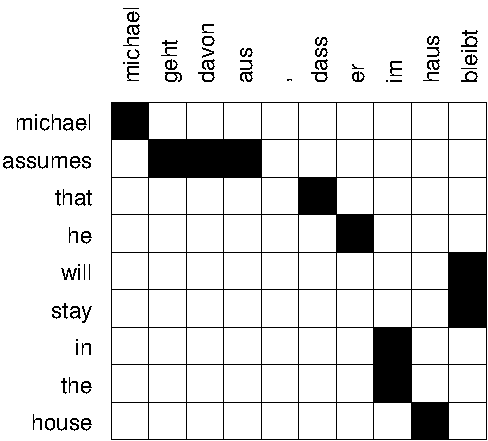
\includegraphics[scale=.8]{figures/michael-alignment.pdf}
\end{center}
\end{frame}


\begin{frame}
\frametitle{Word Alignment?\koehnref}
\vspace{10mm}
\begin{center}
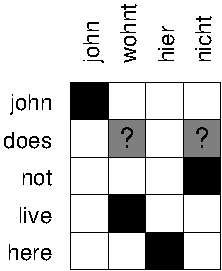
\includegraphics[scale=1.1]{figures/does-not-alignment.pdf}\\[5mm]
Is the English word \textit{does} aligned to\\ the German \textit{wohnt} (verb) or \textit{nicht} (negation) or neither?
\end{center}

\end{frame}


\begin{frame}
\frametitle{Word Alignment?\koehnref}
\vspace{10mm}
\begin{center}
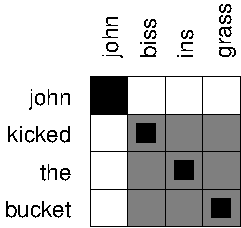
\includegraphics[scale=1.2]{figures/kicked-the-bucket-alignment.pdf}\\[5mm]
How do the idioms \textit{kicked the bucket} and \textit{biss ins grass} match up?\\ Outside this exceptional context, \textit{bucket} is never a good translation for \textit{grass}
\end{center}

\end{frame}


\begin{frame}
\frametitle{Measuring Word Alignment Quality\koehnref}
\vspace{10mm}
\begin{itemize}
\item Manually align corpus with {\em sure} (\maths{$S$}) and {\em possible} (\maths{$P$}) alignment points (\maths{$S \subseteq P$})
\item Common metric for evaluation word alignments: Alignment Error Rate (AER)
\maths{\begin{equation*}
\mbox{AER}(S,P;A) =  \frac{|A \cap S| + {|A \cap P|}}{|A|+|S|}
\end{equation*}}
\item AER = 0: alignment \maths{$A$} matches all sure, any possible alignment points
\item However: different applications require different precision/recall trade-offs
\end{itemize}

\end{frame}


\begin{frame}
\frametitle{Word Alignment with IBM Models\koehnref}

\begin{itemize}
\item IBM Models create a {\bf many-to-one} mapping
{\begin{itemize}\itemsep 3mm
\item words are aligned using an alignment function
\item a function may return the same value for different input
\item[]  (one-to-many mapping)
\item a function can not return multiple values for one input
\item[]  (no many-to-one mapping)
\end{itemize} }
\item  Real word alignments have {\bf many-to-many} mappings
\end{itemize}

\end{frame}


\begin{frame}
\frametitle{Symmetrizing Word Alignments\koehnref}
\vspace{-5mm}
\begin{center} 
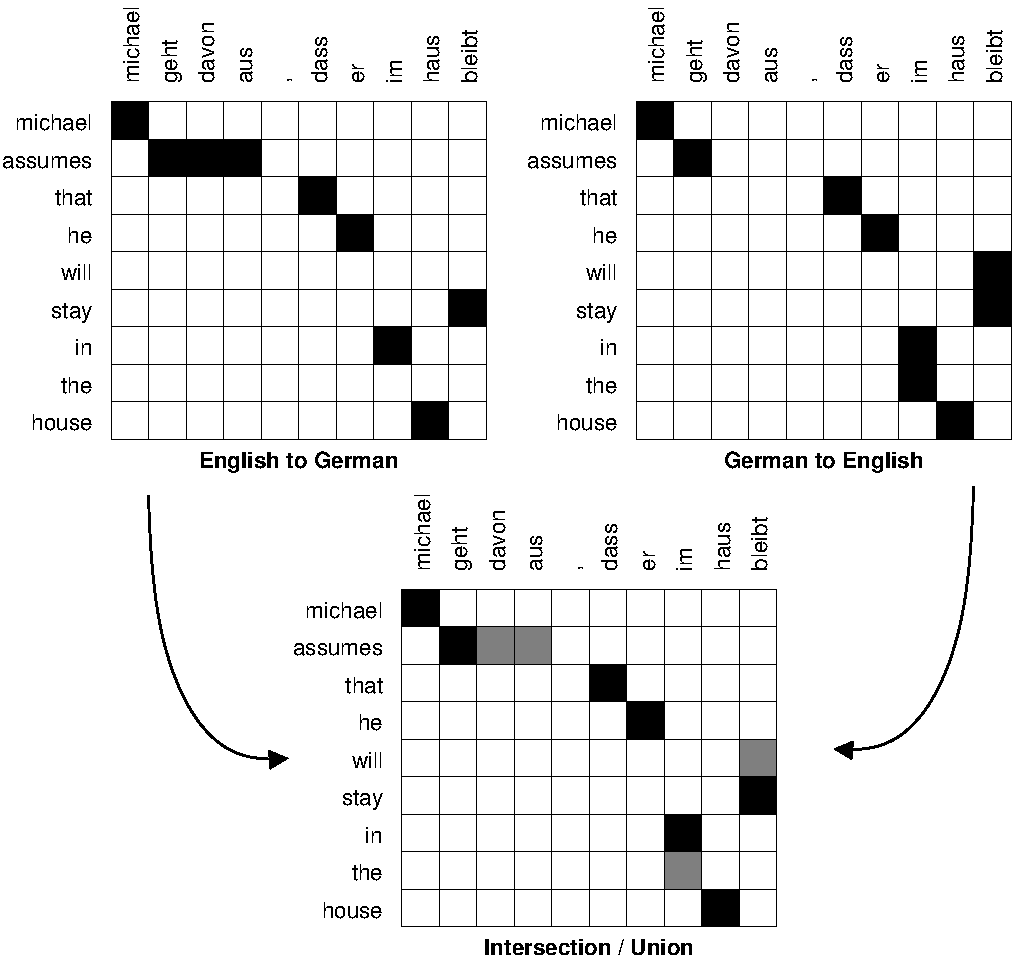
\includegraphics[scale=0.45]{figures/michael-bidirectional.pdf}
\end{center}
\begin{itemize}
\item Intersection plus grow additional alignment points [Och~and~Ney,~CompLing2003]
\end{itemize}

\end{frame}

 
\begin{frame}[fragile]
\frametitle{Growing heuristic\koehnref}

{\footnotesize {\bf grow-diag-final}(e2f,f2e)
\begin{algorithmic}[1]
\STATE neighboring = $\{$(-1,0),(0,-1),(1,0),(0,1),(-1,-1),(-1,1),(1,-1),(1,1)$\}$
\STATE alignment $A$ = intersect(e2f,f2e); grow-diag(); final(e2f); final(f2e);
\end{algorithmic}
{\bf grow-diag}()
\begin{algorithmic}[1]
\WHILE{new points added}
\FORALL{English word $e \in [1 ... e_n]$, foreign word $f \in [1 ... f_n]$, $(e,f) \in A$}
      \FORALL{neighboring alignment points ($e_\text{new}$, $f_\text{new}$)}
         \IF{($e_\text{new}$ unaligned {\sc or} $f_\text{new}$ unaligned) {\sc and} ($e_\text{new},f_\text{new}) \in \text{union(e2f,f2e)}$}
           \STATE add ($e_\text{new},f_\text{new}$) to $A$
        \ENDIF
       \ENDFOR  
  \ENDFOR  
\ENDWHILE
\end{algorithmic}
{\bf final}()
\begin{algorithmic}[1]
\FORALL{English word $e_\text{new} \in [1 ... e_n]$, foreign word $f _\text{new}\in [1 ... f_n]$}
     \IF{($e_\text{new}$ unaligned {\sc or} $f_\text{new}$ unaligned) {\sc and} ($e_\text{new},f_\text{new}) \in \text{union(e2f,f2e)}$}
       \STATE add ($e_\text{new},f_\text{new}$) to $A$
     \ENDIF
\ENDFOR  
\end{algorithmic}
}

\end{frame}

 
\begin{frame}
\frametitle{More Recent Work on Symmetrization\koehnref}

\begin{itemize}
\item Symmetrize after each iteration of IBM Models [Matusov et al., 2004]
\begin{itemize}
\item run one iteration of E-step for each direction
\item symmetrize the two directions
\item count collection (M-step)
\end{itemize}
\vspace{5mm}
\item Use of posterior probabilities in symmetrization 
\begin{itemize}
\item generate n-best alignments for each direction
\item calculate how often an alignment point occurs in these alignments
\item use this posterior probability during symmetrization
\end{itemize}
\end{itemize}

\end{frame}

 
\begin{frame}
\frametitle{Link Deletion / Addition Models\koehnref}

\begin{itemize}
\item Link deletion [Fossum et al., 2008]
\begin{itemize}
\item start with union of IBM Model alignment points
\item delete one alignment point at a time
\item uses a neural network classifiers that also considers aspects such as how useful the alignment is for learning translation rules
\end{itemize}
\vspace{5mm}
\item Link addition [Ren et al., 2007] [Ma et al., 2008]
\begin{itemize}
\item possibly start with a skeleton of highly likely alignment points
\item add one alignment point at a time
\end{itemize}
\end{itemize}

\end{frame}

 
\begin{frame}
\frametitle{Discriminative Training Methods\koehnref}

\begin{itemize}
\item Given some annotated training data, supervised learning methods are possible
\item Structured prediction
\begin{itemize}
\item not just a classification problem
\item solution structure has to be constructed in steps
\end{itemize}
\item Many approaches: maximum entropy, neural networks, support vector machines, conditional random fields, MIRA, ...
\item Small labeled corpus may be used for parameter tuning of unsupervised aligner [Fraser and Marcu, 2007]
\end{itemize}

\end{frame}

 
\begin{frame}
\frametitle{Better Generative Models\koehnref}

\begin{itemize}
\item Aligning phrases
\begin{itemize}
\item joint model [Marcu and Wong, 2002]
\item problem: EM algorithm likes really long phrases
\end{itemize}
\vspace{10mm}
\item Fraser and Marcu: LEAF
\begin{itemize}
\item decomposes word alignment into many steps
\item similar in spirit to IBM Models
\item includes step for grouping into phrase
\end{itemize}
\end{itemize}

\end{frame}


\begin{frame}
\frametitle{Summary\koehnref}
\begin{itemize}
\item Lexical translation
\item Alignment
\item Expectation Maximization (EM) Algorithm
\item Noisy Channel Model
\item IBM Models 1--5
\begin{itemize}
\item IBM Model 1: lexical translation
\item IBM Model 2: alignment model
\item IBM Model 3: fertility
\item IBM Model 4: relative alignment model
\item IBM Model 5: deficiency
\end{itemize}
\item Word Alignment
\end{itemize}

\end{frame}


\section*{Acknowledgements}

\begin{frame}
\centering
\begin{alertblock}{Acknowledgements}
Many slides borrowed or inspired from lecture notes by Michael Collins, Chris Dyer, Kevin Knight, Philipp Koehn, Adam Lopez, Graham Neubig and Luke Zettlemoyer from their NLP course materials. 

\bigskip

All mistakes are my own.

\bigskip

A big thank you to all the students who read through these notes and helped me improve them.

\end{alertblock}
\end{frame}



\end{document}
